\section{System overview of a Real-time Traffic Map}


\begin{figure*}[t!]
\centering
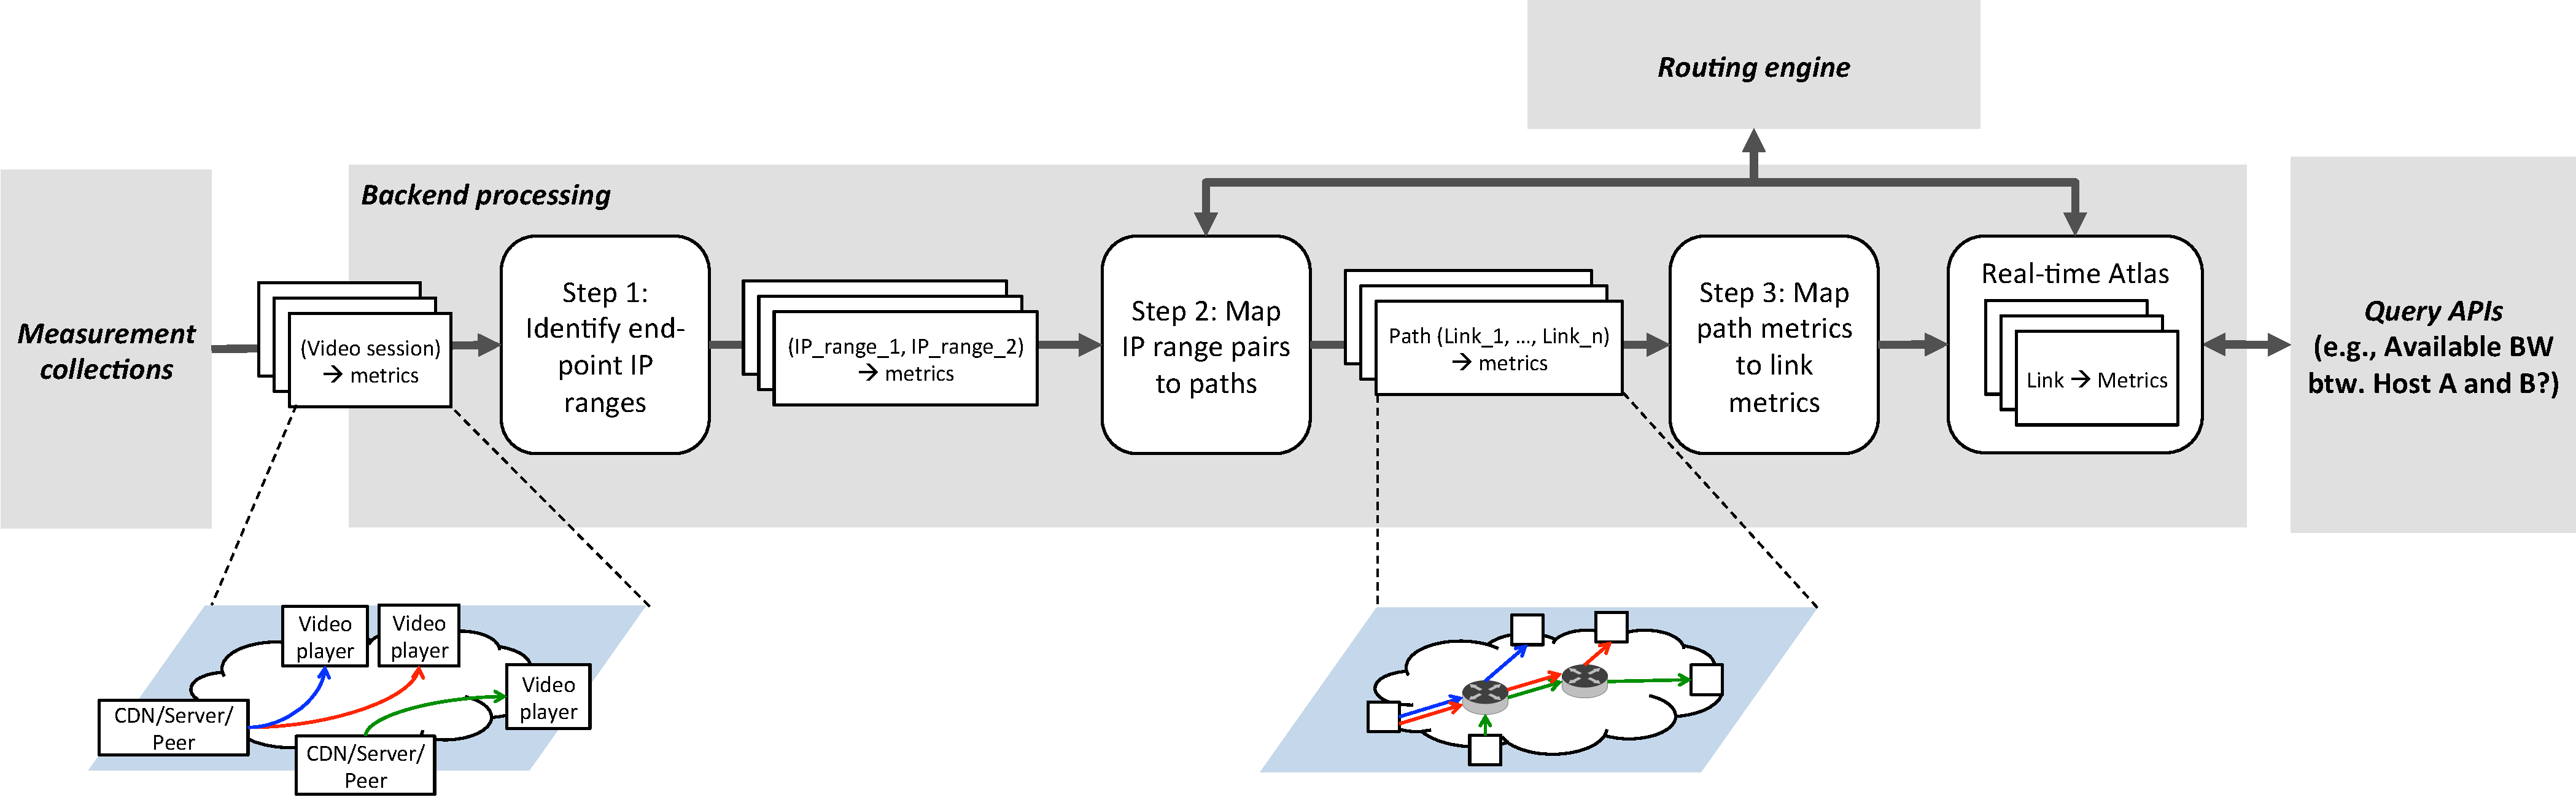
\includegraphics[width=500pt]{figures/system_overview_1.pdf}
\tightcaption{System overview of a Real-time Traffic Map. The {\it measurement engine} gathers raw data of application-layer metrics (e.g., download speed) from client-side video players, and then the {\it backend processing} summarizes the input to get the end-to-end metrics between two hosts, which is mapped to that of paths by querying the {\it routing engine}, and finally converted to an link-annotated topology that can be queried with {\it query APIs}.}
\label{fig:overview:system}
\end{figure*}


The basic function of a Real-time Traffic Map (RTM) is to provide a public service for anyone to query the real-time available bandwidth between two hosts. The system will consist of four high level components -- measurement engine, backend processing, routing engine, and query API. 

\jc{TODO: change the system figure.}

Figure~\ref{fig:overview:system} illustrates the system overview. The {\it measurement engine} gathers raw data of measured application-layer metrics (e.g., download speed) from client-side video players. The measured metrics are associated with the hosts information. The {\it routing engine} provides the path information between any two given hosts. Finally, the {\it backend processing} extrapolates the available bandwidth on each link based on the massive probes from video players.


%Figure~\ref{fig:overview:system} illustrates the system overview. The {\it measurement engine} gathers raw data of application-layer metrics (e.g., download speed) from client-side video players, and then the {\it backend processing} summarizes the input to get the end-to-end metrics between two hosts, which is then mapped to the paths between them by querying the {\it routing engine} and finally converted to an link-annotated topology as an intermediate representation. Such representation is called real-time atlas and can be used to implement the {\it query APIs}. This section presents the interfaces and functionalities of each components, and discusses the challenges in implementing such system.

The our design of RTM provides the technique base for building up such service. In reality, it can be operated by different entities who have access to video player performance. These include video content providers, CDN, or third-party companies. And it has been shown feasible as some companies (e.g., Akamai) have been collecting performance characteristics from video players for different purposes. The coverage of the RTM service operated by different parties may depend on their visibility -- for example, CDN have the view of all traffic from its own servers, while content provider may leverage the opportunities of using multiple CDNs to obtain a different visibility.

This section presents the interfaces and functionalities of each components, and discusses the challenges in implementing such system.

\subsection{Measurement engine}

The measurement engine consists of two parts -- measurement modules running on client-side and a message protocol that determines what to be collect and when to send to backend.

\mypara{Measurement interface} We leverage the software module running on top of multiple streaming protocols (e.g., HDS~\cite{} or HLS~\cite{}) to collect metrics such as download speed. Such module can be found in most of today's Internet video players (e.g., Adobe's OSMF player~\cite{}). It provides interface to access application-layer events such as the time of a video segment being requested, completely retrieved and how many bytes downloaded, and the download speed can be then calculated. So far, we only consider the download speed (i.e., measured available bandwidth) since it is available from most players.

\mypara{Host information} In addition to download speed, the system also needs to obtain the IP information of both client and server side. Most browser-based players today can extrapolate which CDN the server is located from analyzing the URL, and some can even obtain the server IP if the underlying streaming protocol (e.g., RTMP~\cite{}) exposes such knowledge. Finally, the client-side IP is recorded when the player sends the performance statistics back to the backend server.

\mypara{Message protocol} The message protocol decides when and what to be collected from client-side players, and is used as a unified interface between backend and frontend measurement modules running in different players and heterogeneous environments. The protocol also decides whether the message from client-player is pulled by or pushed to back-end server, a decision that could be used for balancing between backend load and information freshness.


\subsection{Backend processing}

The backend processing uses three steps to transform the raw input of measurement engine (i.e., download speed of each current video session) to updates of the ``real-time atlas''.

\mypara{Identify client and server IP ranges (IP/AS/CDN)} Ideally, each video session is associated to a client (destination) and server (source) IP. However, both IPs may inaccurate or incomplete. To tolerate deficient IP information, we attribute them to the most specific {\it IP ranges} among CDN, AS or IP that can be infered from available information. For example, for a session between CDN $A$ (where server AS is unknown) and a client in AS $C$, if based on other sessions, we know that CDN $A$ always uses servers from in AS $B$ to serve clients in AS $C$, we will attribute this session to be from AS $B$ to AS $C$.

\mypara{Map two IP-range to a path} In this step, the routing engine is supposed to provide a routing path given any two IP ranges. 

\mypara{Infer metrics of each link from metrics of all paths} Essentially, it is the most crucial step of the whole system to transfer measured metrics associated to paths to those associated to more basic structural unit (i.e., link) which can be later composed to predict metrics of a path that may have never been probed. It is challenging even if we only consider available bandwidth as the metric to predict for each link. However, it is still feasible to solve by leveraging the massive simulteneous probes from different but overlapping paths. We will present a simple preliminary approach in Section~\ref{sec:idea:pathtolink} that to some extent resolve the challenge.


\subsection{Routing engine}
The routing engine is supposed to be queried with the IP range of source and destination hosts, and predict the link-level path between them. 
Several existing systems provide similar interfaces. For example, iPlane~\cite{} which predicts IP level path by concatenating paths observed in traceroute data. The routing engine is not video-specific and is thus reasonable to rely on other existing systems. However, it is challenging for them (e.g., iPlane) to provide path for all client-server pair in our scenario unless the traffic being measured are similar (e.g., iPlane is based on traceroute between P2P users and does not offer much knowledge on path between CDN servers and clients).

\subsection{Query APIs}


In the most basic form, the RTM query API needs to predict available bandwidth given any two hosts at any time. To this end, the two queried hosts will be first mapped to a path by the routing engine, then the real-time atlas identifies the bottleneck link along the path with the smallest available bandwidth which is then replied as the available bandwdith between the two hosts. 
We also envision the RTM to provide more API by extending the basic API above, including available bandwidth on a link, congestion map, and application-level API such as bottleneck diagnosis and server selection.


\subsection{Challenges}

In a high level, like iPlane, RTM adopts the idea of structural prediction in which a link-annotated map is first generated and the prediction of path performance is made by composing the segments (e.g., links) pre-calculated on the map. However, RTM differs from them in that our input is from the video players which have very limiting available information of network, while previous approaches employ fully controlled machines that can run fine-grain packet-level measurement. Thus, while video offers better coverage and less measurement overhead, we face different set of challenges to make the best of the coarse-grain input.

\mypara{Inferring link-level knowledge from end-to-end performance (corse-grain measured unit)} The end-to-end performance only provides a collective view of all links along it. Specifically, we would like to attribute the end-to-end available bandwidth to the bottleneck link. It becomes more challenging as the available bandwidth measured on each path does not contain packet information which prevent the use of packet dispersion techniques such as Spruce~\cite{}, IGI~\cite{}, Pathload~\cite{}.

\mypara{Inaccurate measured bandwidth (corse-grain measurement results)} The available bandwidth is not measured by packet-level techniques, but relatively long-term download speed. It is well known that the download speed can be affected by packet-level (e.g., TCP window) fluctuation. Moreover, since CDNs always fetch video content from different servers or from a local copy, CDN caching effect can affect the measured download speed.

\mypara{Incomplete IP and path information (corse-grain location knowledge)} Client IP may hehind NAT. Server IP may not be available depending on streaming protocols. Besides, the path predicted by routing engine can be inaccurate or stale.


\mypara{Biased concentration on the network} As more video traffic moves to follow the CDN-client mode, links closer to CDN-side are probed more frequently than those closer to edge. Such skewness requires that the algorithm to generate traffic map has to be not volume-aware, and also poses challenges in predicting between two client hosts.

\mypara{Scalability of back-end} our system has to handle concurrent client-side measurement from \fillme of users, maintain a realtime database for Internet map of \fillme of links, and process large number of queries.


